%Some basic ways to manipulate text are \textit{italics} and \textbf{bold}. One can reference Figures (see Figure \ref{fig:taltech} for an example) as well as cite references which are defined in the \textit{references.bib} file.\cite{spectre,example-reference}
%
%The \textit{Bibliography}, \textit{List of Figures} and \textit{List of Tables} are all automatically generated and references will be updated automatically as well. This means that if you've defined a citation but are not referencing it, it will not appear in the \textit{Bibliography}. This also means that any Figure / Table / Citations numbers are automatically updated as well. Numbering is done by order-of-appearance.
%
%One can create an itemized list:
%\begin{itemize}
%    \item item a
%    \item item b
%    \item ...
%\end{itemize}
%
%Or enumerate them:
%\begin{enumerate}
%    \item item x
%    \item item y
%    \item ...
%\end{enumerate}
%
%
%\begin{figure}[ht]
%    \centering
%    
\includegraphics[width=.5\textwidth]{figures/taltech.jpg}
%    \caption{\textit{An image of the TalTech logo.}}
%    \label{fig:taltech}
%\end{figure}
%
%
%A table with three columns can be seen in Table \ref{tab:requirements}.
%\begin{longtable}{|p{0,5cm}|p{10cm}|p{3cm}|}
%	\caption{\it{A table with some requirements}}
%	\label{tab:requirements}\\ \hline
%	\textbf{Nr} &  \textbf{Requirement} & \textbf{Weight}  \\
%	\hline
%	\endfirsthead
%	\multicolumn{3}{l}%
%	{\tablename\ \thetable\ -- \textit{Continues...}} \\ q
%	\hline
%	\textbf{Nr} &  \textbf{Requirement} & \textbf{Importance}  \\
%	\hline
%	\endhead
%	\hline \multicolumn{3}{l}{\textit{Continues...}} \\
%	\endfoot
%	\hline
%	\endlastfoot
%1 & Price & High\\ \hline
%2 & Variety& Middle\\ \hline
%3 & Support& Low\\ \hline
%
%\end{longtable}
%
%We can use variables set in the \textit{main.tex} file to render values like our title (\doctitle) or supervisor names (\textbf{Supervisor}: \supervisor, \textbf{Co-supervisor}: \cosupervisor{}).
%\section{What is a stream processing}\label{sec:stream-beg}
%Stream processing
%
%\section{Brief history of stream processing systems}\label{sec:breif-history}
%Stream processing


\section{Background and motivation}\label{sec:back-and-motiv}
A necessity in choosing the best suitable technology stack and a framework is
coming from a rapid growth of different kind of data sources which produce
a large volumes of data in a real time.
A definition of big data volumes has changed over time, and it's only growing.
The use case which is considered in this research is supposed to work with a
1TB of data per day, and it's obviously that in some time, for example, in
a couple of years 1TB might be won't be sufficient.
Another perspective of the first is to get an overview of open sources solutions
which could be successfully applied for appropriate use case.
Writing a custom big data framework would require too much effort,
and there's no guarantee that it will reach the same performance.
Obviously, if such framework could be written in assembly language,
which provide the best performance it wouldn't be possible to integrate
to a java based technology stack.
Fortunately, an open source community has grown a lot over the last years
and provides grate tooling for many use cases.
Considering open source solutions for a big data.

\newpage
\section{Problem statement}\label{sec:prob-st}
The problem is coming with a business demands which are based on a current needs
for a more scalable and efficient solution.
Before getting into a problem details, the current model will be provided, to
get better understanding why this research brings value and how streaming frameworks
are comparable with the current model.

\subsection{Current model overview}\label{subsec:current-model}

\begin{figure}[ht]
    \centering
    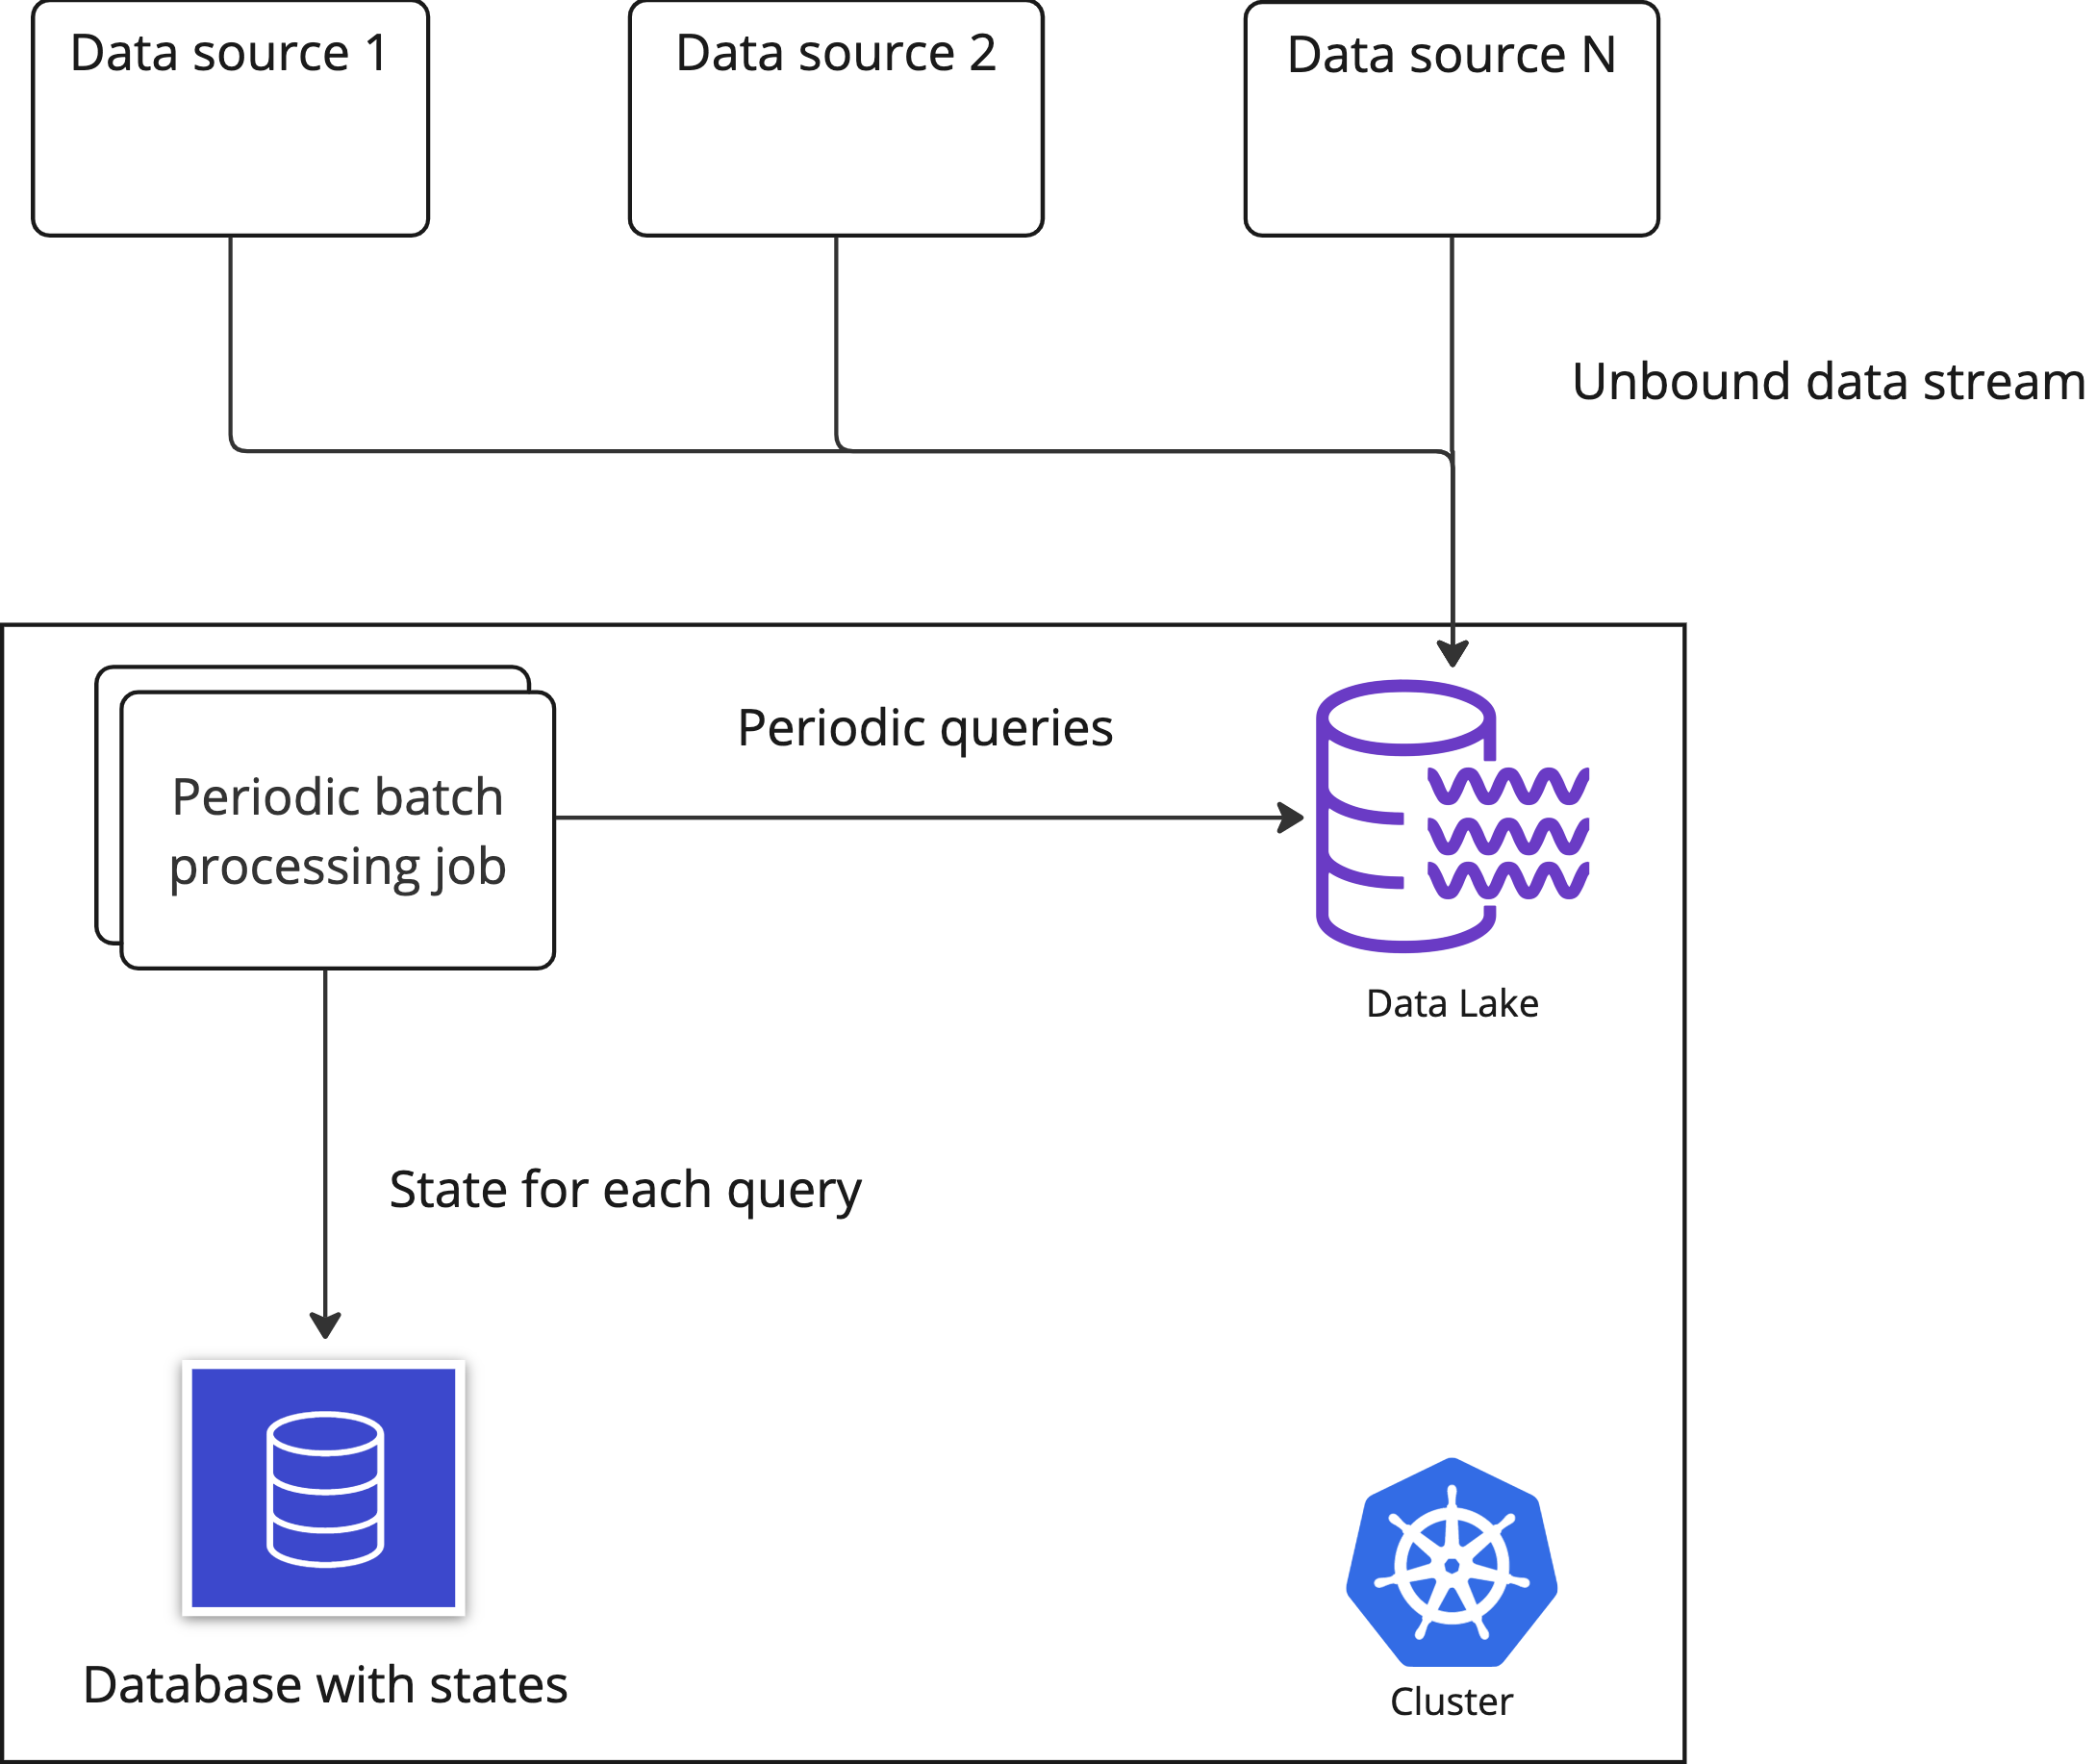
\includegraphics[width=.5\textwidth]{figures/current-model}
    \caption{\textit{Generic model of current data processing system.}}
    \label{fig:current-model}
\end{figure}

The figure\ref{fig:current-model} represents only a very generic model of the current
system to just get some overview.
The model contain the following components.

\begin{description}
    \item[Kubernetes cluster] An environment for cluster components.
    \item[Data course N] Is an external component which sends a data messages in unbound mode.
    Each data source is located in different external network and gets connected through
    a network gateway before it reaches the job.
    Each data messages gets saved in a data lake.
    \item[Processing job] Represents a functionality block which uses queries to access the
    data lake and save intermediate state to the state database.
    The job represents an application written in highly-level object-oriented programming language like Java, C\#
    and works in a batch processing mode which means it gets launched periodically.
    \item[Databse with states] Contains states for queries, a state is a crucial part of the job's pipeline.
    Contains an information from previous query executions.
    \item[Date late] Is a central data storage which provides a query interface.
\end{description}

From a first look, the system which is on the Figure \ref{fig:current-model} defines a straightforward
architecture.
Generally, the systems which implements such architecture are easily debuggable,
testable and quite often is a good way to go when the project gets started.
Everything might work smoothly for ages.
At some moment in time, the system might face with a breaking point which brings new challenges.

For example, in a few years, the number of data sources has significantly grown, where each
data source has its own sending frequency and a type.
A new load would require to add more and more instances of a job, faster period of job execution.
And also it leads to additional types of errors to handle, which haven't been seen before.
An execution of each query gets more expensive.
Not every data can be indexed, and especially if amount of indexed data has grown in many times, it adds
a significant complexity overhead for a query execution.
Moreover, additional errors might and circumstances may get the service down, which requires
additional balancing logic and a state recovery.
At might take a significant time to recover a service in specific region if this requires a manual work
from engineering team.

As a summary, some crucial problems can be defined as follows.

\begin{itemize}
    \item The system is not scalable enough.
    \item A state is lost after recovery, not completely fault tolerant.
    \item Expensive query execution, especially if data is not indexed
    \item Job processing is periodic, leads to a latency and limitation in processing time.
\end{itemize}

\newpage
\section{Research question and objectives}\label{sec:res-q-o}
Based on given description it's possible to set objectives and direction
where thesis research should be directed.
Obviously, that based on given major problems given as bullet points in previous section
some other sub problems appear which must considered in this research.

\subsection{Alternative architectures}\label{subsec:alternative-architectures-and-frameworks}
Fortunately, similar problems have already known in IT industry and big players like Google, Microsoft
have invested enough resources.
Their research results lead to a stream processing.
Stream processing is tend to be as alternative for bach processing which works for most cases, but
this specific use case if focused on real time data.
Once it's clear that stream processing is the way to go then comes a next question.
Another solution is to come up with a custom solution.
However, the most significant disadvantages include:

\begin{itemize}
    \item A need to hire a team just to developer another stream processing framework.
    \item There's a big change that a custom solution won't perform better than existing.
    \item Long-term engineering support, such as bug fixes, integration with external dependencies,
    feature development.
    \item The cost can become prohibitive.
\end{itemize}


At the same time, the open source community is huge enough, which supports the greatest
open source products under The Apache Software Foundation.
The most significant disadvantages include:

\begin{itemize}
    \item Industry standard frameworks.
    \item A huge support from developer around the world.
    \item An ease in extending already made code.
    \item Lots of ready for use tutorials and documentations.
    \item Many examples for different use cases.
\end{itemize}


\newpage
\subsection{Selecting a suitable framework}\label{subsec:selecting-a-suitable-framework}
They're lots different frameworks out there available for solving different
data streaming problems.
Most of the were born on top of each other as a new generation solution.
Each new framework is trying to bring better performance and scalability.
Down below is an evolution of streaming frameworks with a brief description:

\begin{description}
    \item[Apache S4 (2010)]  Apache S4 (Simple Scalable Streaming System) was an early stream
    processing engine developed at Yahoo! Labs.
    It was designed for unbounded data stream processing which uses
    simple programming model based on a publish/subscribe pattern.
    Apache S4 became an open source project under Apache Software Foundation but
    eventually became inactive due to limited community adoption.
    \item[Apache Storm (2011)]
    Apache Storm was a popular distributed stream processing framework.
    It was designed for real-time data processing and provided guarantees such as
    at-least-once and exactly-once processing semantics.
    Apache Storm was more popular comparing to Apache S4, but it provides less
    performance and flexibility comparing to next generation frameworks.
    \item[Apache Samza (2013)] Samza was developed at LinkedIn, as another distributed stream processing.
    Samza provided better integration for Kafka,
    offering strong durability guarantees and support for stateful stream processing.
    Samza also allowed users to perform windowed operations and join streams with external data stores.
    In general, Samza is a base for a next generation stream processing framework which called Kafka streams.
    \item[Apache Flink (2014)] Originally was developed at the Technical University of Berlin.
    Apache Flink is one of the most powerful stream processing framework that unified batch and
    stream processing with focusing on streaming.
    Flink provided low-latency, high-throughput, and exactly-once processing semantics.
    With its advanced features, such as event time processing, watermarks, and savepoints,
    Flink has become the one of the most popular stream processing framework which is
    well-designed for highly loaded complex data stream processing use cases.
    \item[Apache Kafka Streams (2016)] Introduced as part of Apache Kafka, Kafka Streams
    is a rather a stream processing library than a framework which allows developers to build real-time
    applications and microservices using the Kafka platform.
    Kafka Streams provides a simple, functional programming model and is tightly
    integrated with the Kafka ecosystem.
    It's well-suited for use cases like real-time analytics, data transformation
    and event-driven architectures.
    Kafka Stream can a replacement for Apache Flink for cases where heavy integration
    and complex computation is not needed.
    \item[Apache Beam (2016)] In general, provides an abstraction layer that allows
    jobs to run on top of other data processing engines such as Apache Spark, Apache Flink and
    Google Cloud Dataflow since it was developed by Google.
    It might bring a performance overhead for heavily loaded jobs.
\end{description}

There's another open source framework which is called Apache Spark.
Apache Spark is great tool for many cases, but it's better adjusted
for a batch processing which would work good enough for most other use cases.

As we see from the list above, even during last 10 years quite many different frameworks have
been released, and who knows what else to expect in a near future.
At least two Apache Flink and Kafka streams are well-designed for
complex stateful stream processing.
Also, both have a great open source community support.
However, some companies fork these projects to add additional features for their use cases.

\subsection{Deployment environment}\label{subsec:deployment-environment}
In 2023 the most popular and advanced application container manager is Kubernetes.
First stream processing frameworks were adopted to be running on YARN clusters.
YARN is not considered to be preferable deployment manager anymore.
It means that a framework must be able to run in Kubernetes using containers.


\subsection{Benchmarking}\label{subsec:bench}
Benchmarking is an additional problem that has to be solved.
There are lots of different benchmarks are already available, which can
be taken into account, but obviously there is no benchmarks for considered use case.

\subsection{Requirements summary}\label{subsec:final-requirements}
At the moment, there are two leading frameworks are available which
should help to build efficient and reliable solution, and
they are Apache Flink and Kafka Streams.
Both are designed for data streaming problems, have a large community support.
More detailed comparison will are described in the next section.

As a summary, these important bullet points provided down below which will
be considered during the evaluation for the new solution.

\begin{description}
    \item[Scalability] The current is not scalable enough.
    \item[Fault tolerance] A state must not be lost if a pod where job is running got down,
    the system should be able to proceed processing with previous state once job is recovered.
    \item[Simple integration] A solution, weather it is a programming language,
    or framework, should be compatible with the current technology stack, such as JVM and Kubernetes.
    It also means that a solution won't require hiring an entire engineering department or a team.
    \item[Cost effecienty] It's quite important that a highly loaded solution doesn't cost too much.
    \item[Cloud independence] A solution must not depend on a cloud provider.
    \item[Functionality] A solution has to have an API which allows to implement and test a considered use case.
\end{description}


